\documentclass{beamer}

\usepackage[utf8x]{inputenc}
\usepackage[LGR,T1]{fontenc}
% \usepackage{lmodern}

\usepackage{fancybox}
\usepackage{url}
\usepackage{multirow}
\usepackage[makeroom]{cancel}
\usepackage{ulem}
\usepackage{ifthen}
\usepackage{pgf}
% \usepackage{times}
% \usepackage[T1]{fontenc}
\usepackage{amsthm,amsmath}
\usepackage{etex}
\usepackage{ulem}
\usepackage{tabularx}
\usepackage{graphicx}
\usepackage{listings}
\usepackage{bussproofs}

\usepackage{cmap}
% \usepackage{fontspec}

\usepackage[Bjarne]{fncychap}


\usepackage{tikz}
% \usetikzlibrary{shapes,backgrounds,arrows,automata,positioning,calc}
% \tikzset{
%   modal/.style={>=stealth',shorten >=1pt,shorten <=1pt,auto,node distance=1.5cm,
%     semithick},
%   world/.style={circle,draw,minimum size=0.5cm,fill=gray!15},
%   point/.style={circle,draw,inner sep=0.5mm,fill=black},
%   reflexive above/.style={->,loop,looseness=7,in=120,out=60},
%   reflexive below/.style={->,loop,looseness=7,in=240,out=300},
%   reflexive left/.style={->,loop,looseness=7,in=150,out=210},
%   reflexive right/.style={->,loop,looseness=7,in=30,out=330}
% }


\hypersetup{
    colorlinks=true,
    linkcolor=blue,
    filecolor=magenta,
    urlcolor=cyan}

\lstdefinelanguage{plist}{
  columns=fullflexible,
  upquote=true,
  basicstyle=\rmfamily,
  commentstyle=\ttfamily\itshape\color{green!50!black},
  morestring=[s]{"}{"},
  stringstyle=\color{blue},
  keywords={:pos,:tokens,\:gloss},
  inputencoding=utf8,
  keywordstyle=\bfseries\color{violet}}

\definecolor{ceruleanblue}{rgb}{0.16, 0.32, 0.75}

\usepackage{color}
\definecolor{keywordcolor}{rgb}{0.7, 0.1, 0.1}   % red
\definecolor{commentcolor}{rgb}{0.4, 0.4, 0.4}   % grey
\definecolor{symbolcolor}{rgb}{0.0, 0.1, 0.6}    % blue
\definecolor{sortcolor}{rgb}{0.1, 0.5, 0.1}      % green
\definecolor{errorcolor}{rgb}{1, 0, 0}           % bright red
\definecolor{stringcolor}{rgb}{0.5, 0.3, 0.2}    % brown
\definecolor{yellow}{RGB}{240,228,66}

\usepackage{listings}

\title{Lógica Proposicional e Dedução Natural \\ 
 Matemática Discreta - EMAp/FGV}
\author{Alexandre Rademaker}

\newcommand{\rl}[1]{\RightLabel{\small #1}}

% %% code for listing all frame titles
% \newif\ifframeinlbf
% \frameinlbftrue
% \makeatletter
% \newcommand\listofframes{\@starttoc{lbf}}
% \makeatother

% \addtobeamertemplate{frametitle}{}{%
%   \ifframeinlbf
%   \addcontentsline{lbf}{section}{\protect\makebox[2em][l]{%
%     \protect\usebeamercolor[fg]{structure}\insertframenumber\hfill}%
%   \insertframetitle\par}%
%   \else\fi
% }

\AtBeginSection[]
{
  % \usebackgroundtemplate{\includegraphics[width=\paperwidth]{IMG_1032.jpeg}}
  % \setbeamercolor{background canvas}{bg=yellow}
  % \setbeamercolor{normal text}{fg=black}
  % \setbeamercolor{title}{fg=black}
  % \usebeamercolor[fg]{normal text}
  % \setbeamertemplate{background canvas}[bg]
  \begin{frame}
    \frametitle{Roadmap}
    \tableofcontents[currentsection]
  \end{frame}
  % \usebackgroundtemplate{}
  % \setbeamercolor{background canvas}{bg=yellow}
  % \setbeamercolor{normal text}{fg=black}
  % \setbeamertemplate{background canvas}[bg]
  % \setbeamercolor{frametitle}{fg=ceruleanblue}
  % \usebeamercolor[fg]{normal text}
}


\newenvironment{wideitemize}{\itemize\addtolength{\itemsep}{10pt}}{\enditemize}


\begin{document}

\usebackgroundtemplate{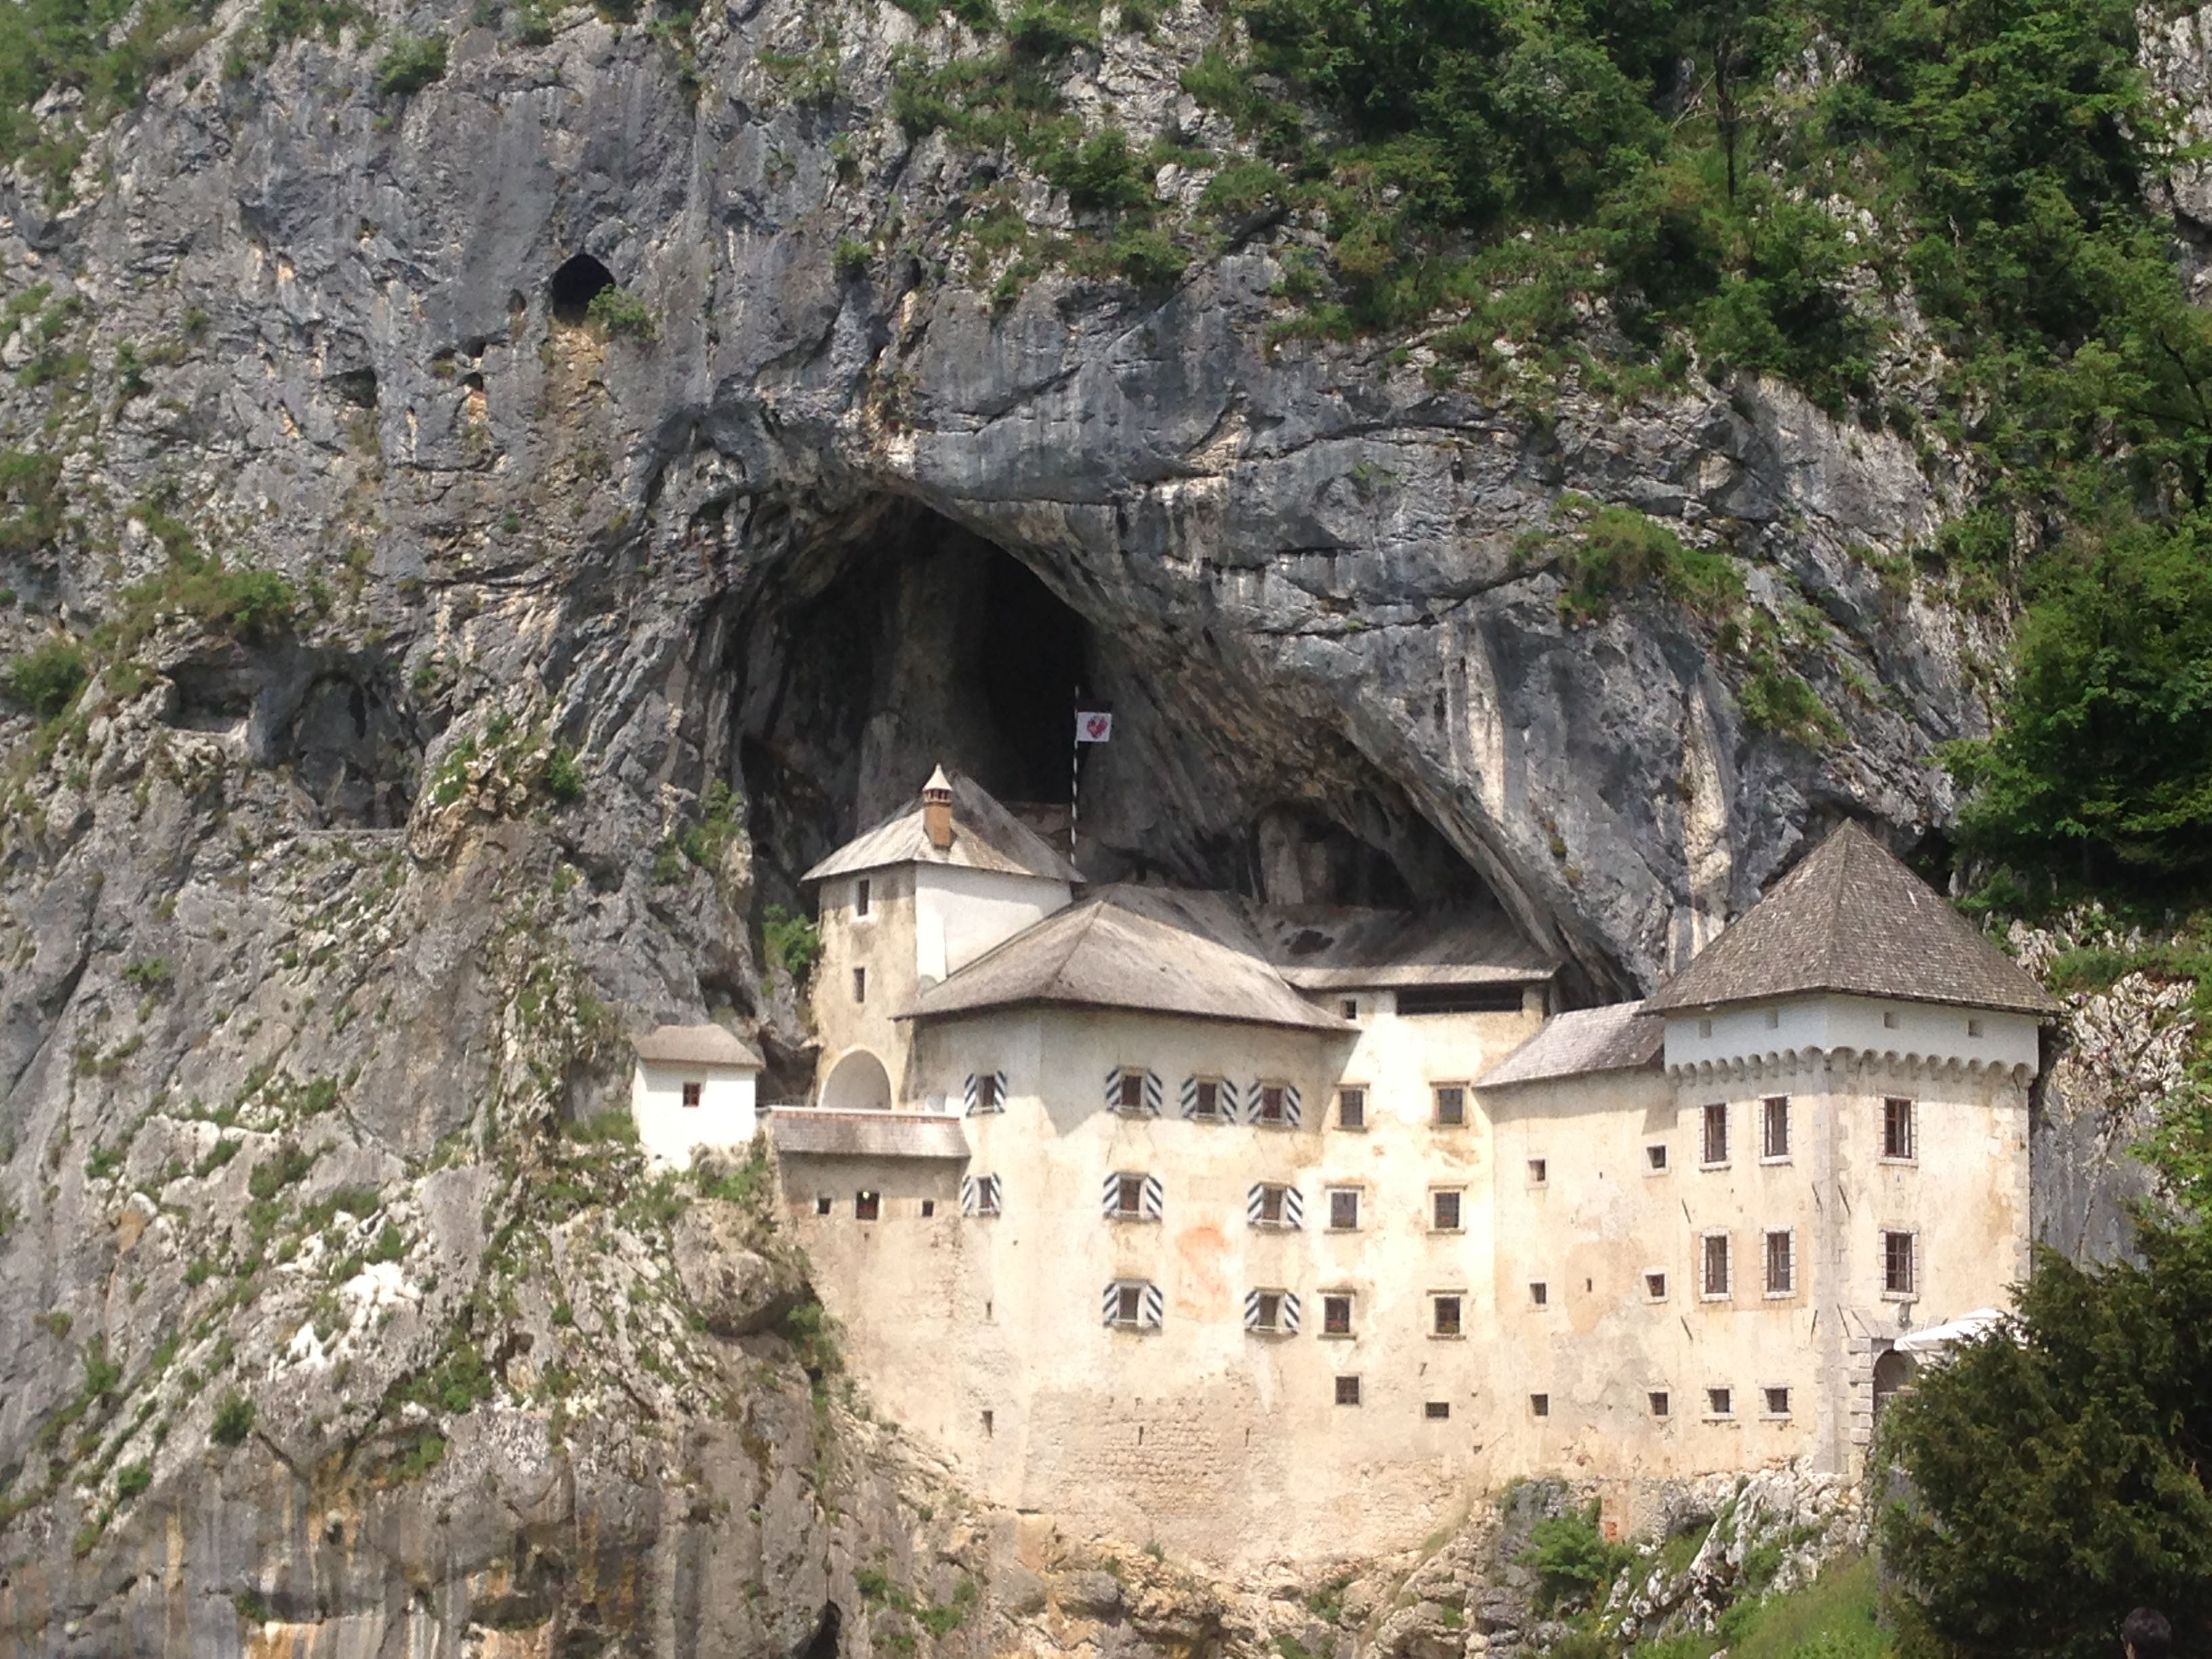
\includegraphics[width=\paperwidth]{IMG_0318.jpeg}}
\setbeamercolor{normal text}{fg=white}
\setbeamercolor{title}{fg=white}
\usebeamercolor[fg]{normal text}
\frame{\titlepage}
\usebackgroundtemplate{}
\setbeamercolor{normal text}{fg=black}
\setbeamercolor{frametitle}{fg=ceruleanblue}
\usebeamercolor[fg]{normal text}

\section{Asymptotic notation}


\begin{frame}[fragile]{Asymptotic notations}

  $\Theta$, $O$, and $\Omega$ (‘big theta’, ‘big omicron’, and ‘big
  omega’).\\~\

  $f = \Theta(g)$ f is of order of g.\\~\

  $f = O(g)$ f is of order at most g.\\~\

  $f = \Omega(g)$ f is of otder at least g.

\end{frame}

\begin{frame}{Big Theta}
  We say that $f$ is of order $g$, and write $f = \Theta(g)$, if there
  are positive constants $C$ and $D$ and a number $n_0$ such that, for
  all $n > n_0$,
  \[ Cg(n) \leq f(n) \leq D g(n) \] 
  
  Examples
  \begin{equation*}
    \begin{split}
      n(n+1)/2 &=\Theta(n^2)\\
      n^3 +n^2 + n log n &= \Theta(n^3)\\
      n (1+1/2+1/3+\ldots) &= \Theta(n log n)
    \end{split}
  \end{equation*}\\~\

  We write $f(n) = \Theta(g(n))$ or $f = \Theta(g)$ or $f \in \Theta(g)$.\\~\

  Example: $head(list)$, it is $\Theta(1)$.
\end{frame}

\begin{frame}{Big Omicron}
  We say that $f$ is of order at most $g$, and write $f = O(g)$, if there
  are positive constants $C$ and a number $n_0$ such that, for
  all $n > n_0$,
  \[ f(n) \leq C g(n) \]

  In particular, $O(1)$ stands for an anonymous function whose values
  are bounded above by some positive constant.\\~\

  The running time of $takeWhile$ on a list of length $n$ is $O(n)$
  steps, assuming the test takes constant time.\\~\

  In the \emph{worst case} the running time is $\Theta(n)$ steps but in the
  best case, when the first element does not pass the test, the
  running time is $\Theta(1)$ steps.
\end{frame}

\begin{frame}{Big Omega}
  A running time of $O(n^2)$ does not imply that the running time is not
  also $O(n)$.\\~\

  We say that f is of order at least g, and write $f = \Omega(g)$, if
  there is a positive constant $C$ and a natural number $n_0$ such that
  \[ f(n) \geq C g(n)\]\\~\

  It follows that $f=\Theta(g)$ if and only if $f=O(g)$ and
  $f =\Omega(g)$.
\end{frame}



\end{document}


  
%%% Local Variables:
%%% mode: latex
%%% TeX-master: t
%%% End:
